% !Mode:: "TeX:UTF-8"
% !Mode:: "TeX:UTF-8"
\newcommand{\thepage}{} % to silence a hyperref warning about pdfpagelabels
\RequirePackage[]{silence}
\WarningsOff[hyperref]
\PassOptionsToPackage{log-declarations=false}{xparse}
%\RequirePackage[l2tabu, orthodox]{nag}
\RequirePackage{luatex85} % to make \pdf...= commands work with LuaTeX
\documentclass[aspectratio=169,t]{beamer}
\usepackage{ifthen}
\usepackage[T1]{fontenc}
\usepackage{iftex}
\ifLuaTeX
 \usepackage{fontspec}
 \setmainfont[Ligatures=TeX]{Source Sans Pro}
\else
 \usepackage[utf8]{inputenc}
\fi
\usepackage{german}
\usepackage{newunicodechar}
\newunicodechar{€}{\texteuro}
\newunicodechar{ß}{\ss}
\renewcommand{\SS}{\iffontchar\font"1E9E \symbol{"1E9E}\else SS\fi}
\usepackage{ellipsis}
\usepackage{microtype}
\usepackage{listings}
\usepackage{sourcecodepro}
\lstset{language=Python, basicstyle=\ttfamily}
\usepackage{amsfonts}
\usepackage{amssymb}
\usepackage{amsthm}
\usepackage{fancyhdr}
\usepackage{graphicx}

\newtheorem{proposition}[theorem]{Proposition}

\DeclareMathOperator*{\argmax}{argmax}
\DeclareMathOperator{\supp}{supp}
\newcommand{\E}{\ensuremath{\mathbb{E}}}
\newcommand{\V}{\ensuremath{\mathbb{V}}}

\setbeamercolor{emph}{fg=purple}
\renewcommand<>{\emph}[1]{%
  {\usebeamercolor[fg]{emph}\only#2{\itshape}#1}%
}



\hypersetup{draft=false,colorlinks=false,pdfpagemode=UseOutlines,plainpages=false,
            breaklinks=true,bookmarksnumbered=true,pdfborder=0 0 0,
            pdftitle={Data Science SoSe 2026 HHU},
            pdfauthor={Konrad Voelkel},
            pdfsubject={data science}}

%\documentclass[aspectratio=169,t]{beamer}
\usetheme{hhubeamer} % put the hhu-beamer-theme in /usr/share/texmf/tex/latex/beamer/themes/

% -------------------- Code listings config --------------------
% Define custom colors for syntax highlighting
\definecolor{codegreen}{rgb}{0,0.6,0}
\definecolor{codegray}{rgb}{0.5,0.5,0.5}
\definecolor{codepurple}{rgb}{0.58,0,0.82}
\definecolor{backcolour}{rgb}{0.96,0.96,0.94} % Very light gray/beige
% Configure the listings package
\lstset{
    language=Python,
    backgroundcolor=\color{backcolour},   
    commentstyle=\color{codegreen}\itshape,
    keywordstyle=\color{blue}\bfseries,
    numberstyle=\tiny\color{codegray},
    stringstyle=\color{codepurple},
    basicstyle=\ttfamily\footnotesize, % Use a monospaced font
    breakatwhitespace=false,         
    breaklines=true,      
             % Enable automatic line breaking
    captionpos=b,                      % Caption at the bottom
    keepspaces=true,                 
    numbers=left,                      % Line numbers on the left
    numbersep=10pt,                    % Distance of line numbers from the code
    showspaces=false,                
    showstringspaces=false,            % Don't show weird underscores in strings
    showtabs=false,                  
    tabsize=4,
    frame=single,                      % Add a subtle border around the code
    rulecolor=\color{black!20},        % Border color
  }

\event[]{}
\author[Sommersemester 2026]{Dr. Konrad Völkel, Sommersemester 2026}

%\title{Data Science, VL 1}
%\date{16.04.2026}


%%% Local Variables:
%%% mode: latex
%%% TeX-master: t
%%% End:


\title{Data Science, VL 6} % war in 2025 noch VL 5; Einschub zu Python kam dazwischen...
\subtitle{Diskrete Verteilungen}
\date{07.05.2026}

\newcommand{\ceil}[1]{\ensuremath{\left\lceil #1 \right\rceil}}

\begin{document}

\begin{frame}
  \titlepage
\end{frame}

\section{Entropie}

\begin{frame}
  \frametitle{Entropie}
  \framesubtitle{Was ist das?}
  \begin{center}
    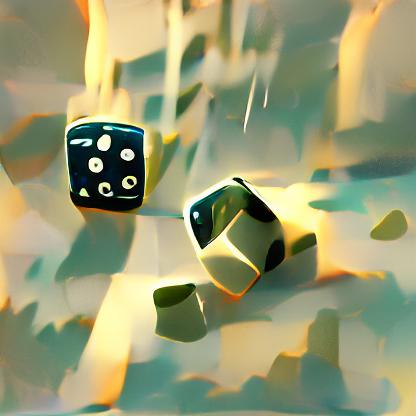
\includegraphics[height=0.7\textheight]{figures/falling_dice.jpg} \\
    \small ``Falling dice''
  \end{center}
\end{frame}

\begin{frame}
  \frametitle{Was ist Entropie - in der Physik}
  \framesubtitle{Das Standardbeispiel}
  Wir vergleichen zwei exakt gleich beschaffene Container mit Gas drin. \\
  Exakt gleich viele Gasteilchen.
  
      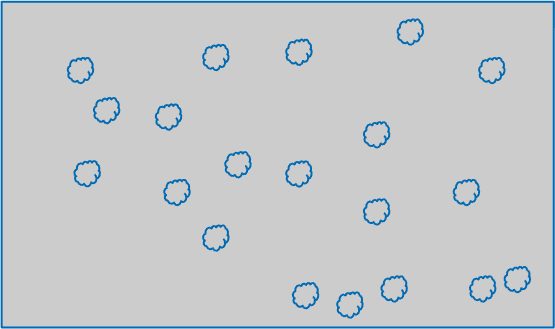
\includegraphics[width=.34\textwidth]{figures/gas_container_high_entropy.png}
      \hspace{0.5cm}
      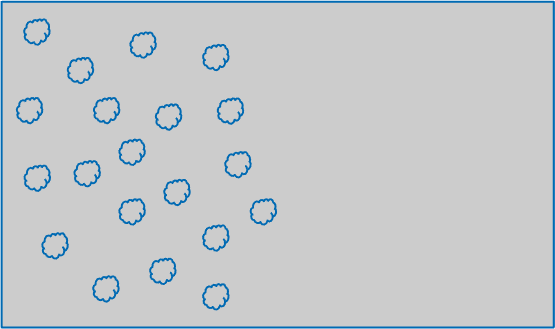
\includegraphics[width=.34\textwidth]{figures/gas_container_low_entropy.png}

      
      \begin{itemize}[<+->]
        \item Was überrascht uns mehr? \alert{Rechts.}
        \item Was wird passieren? \alert{Es sieht bald aus wie links.}
        \item Links: \alert{hohe Entropie}
        \item Rechts: \alert{niedrige Entropie}
        \item \vspace{-4cm} \textbf{2. Hauptsatz der Thermodynamik:}\\ In einem geschlossenen adiabaten System kann die Entropie nicht geringer werden. (Das System tauscht keine Wärme mit der Umgebung aus.) \vspace{4cm}
        \end{itemize}
        
\end{frame}

\begin{frame}
  \frametitle{2. Hauptsatz der Thermodynamik für Dummies}
  \begin{center}
    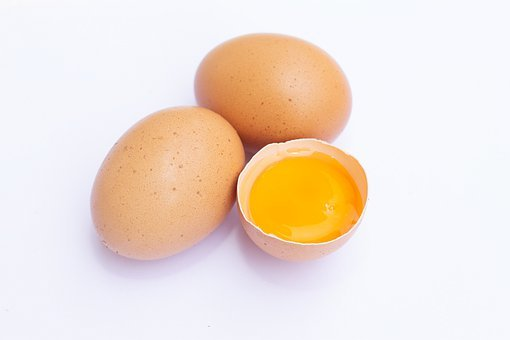
\includegraphics[width=0.4\textwidth]{figures/raw_eggs.jpg}
    \hspace{1cm}
    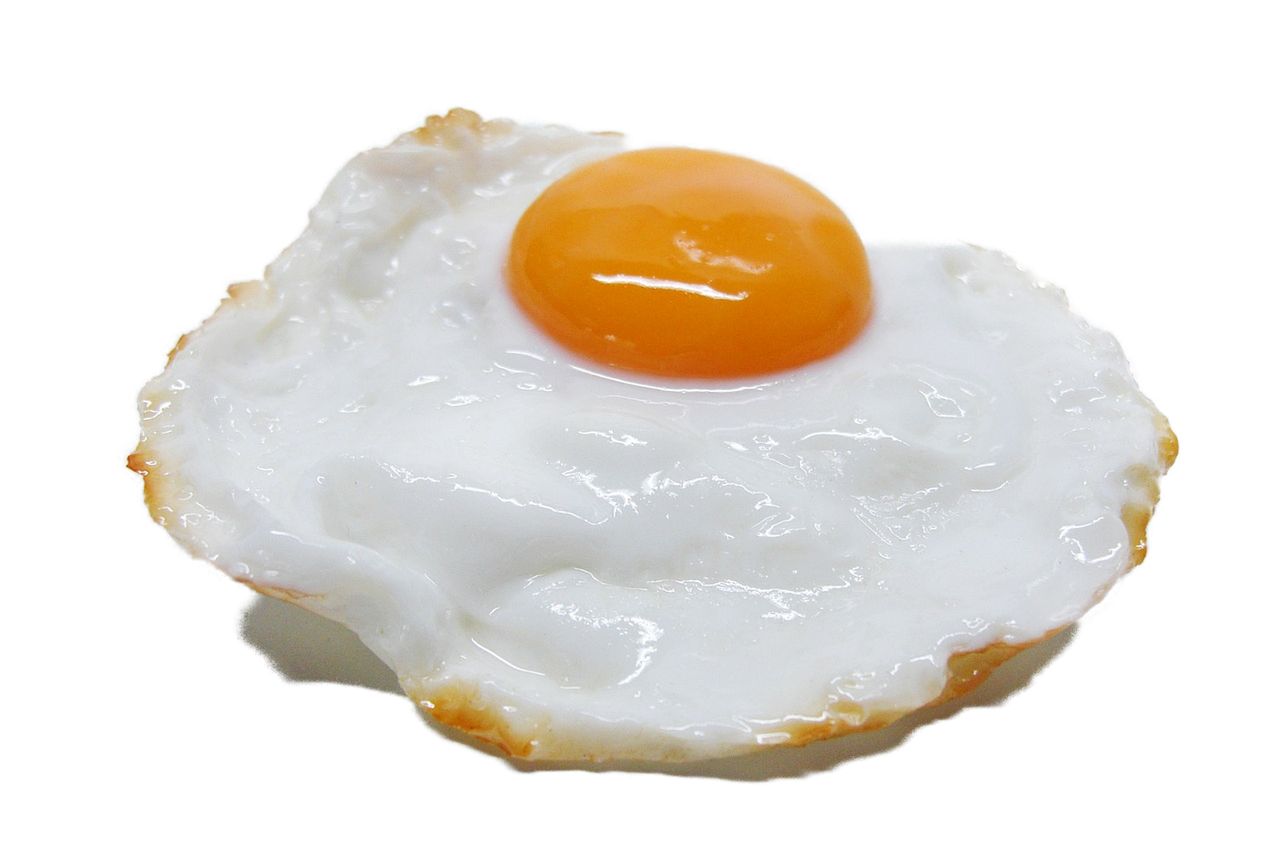
\includegraphics[width=0.4\textwidth]{figures/fried_egg.png}\\
    \vspace{0.5cm}
    \uncover<2->{\alert{Das geht nur in eine Richtung!}}
  \end{center}
\end{frame}

\begin{frame}
  \frametitle{Was ist Entropie - in der Physik}
  Der Unterschied der Container wird besonders sichtbar,\\ wenn man eine Grenze einzieht:
  \begin{columns}
    \begin{column}{0.5\textwidth}
      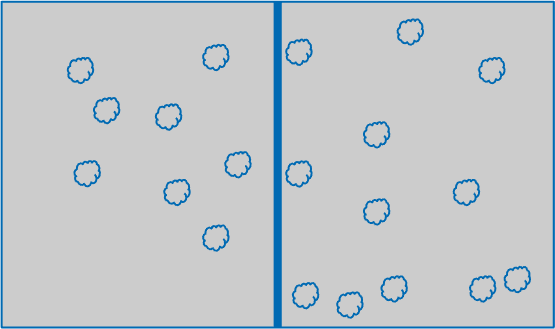
\includegraphics[width=\textwidth]{figures/gas_container_split_high_entropy.png} \\
      \begin{center}hohe Entropie\end{center}
    \end{column}
    \begin{column}{0.5\textwidth}
      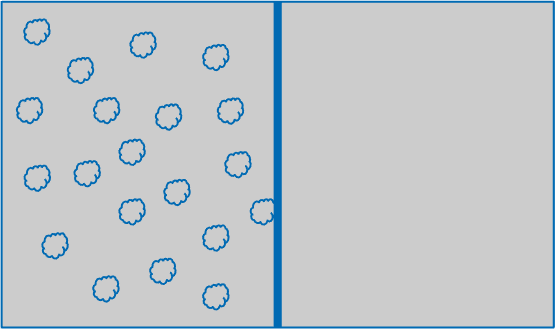
\includegraphics[width=\textwidth]{figures/gas_container_split_low_entropy.png} \\
      \begin{center}niedrige Entropie\end{center}
    \end{column}
  \end{columns}
  \vspace{0.5cm}
  \uncover<2->{
    \begin{itemize}
      \item Entropie = Unordnung? Nicht ganz...
      \item $\Rightarrow$ \alert{Mikrozustände vs. Makrozustände}
      \item Makrozustand ist fix bei beiden Containern.
      \item Mikrozustand jedes Teilchens hat verschieden viele Möglichkeiten.
    \end{itemize}
  }
\end{frame}

\begin{frame}
  \frametitle{Was ist Entropie - in der Physik}
  \textbf{Boltzmann:} In einem abgeschlossenen System mit festem Volumen und fixer Teilchenzahl ist die Entropie proportional zum Logarithmus der Anzahl von Mikrozuständen in dem System.

  \begin{itemize}[<+->]
    \item Mikrozustände sind alle Möglichkeiten, wie sich die Teilchen des eingesperrten Gases anordnen können.
    \item \textbf{Wir merken uns:} Die Entropie ist relativ zu einem Makrozustand definiert, also was wir im ``Großen'' erwarten. Es geht um die Verteilung im ``Kleinen''.
    \item Wir zählen und nehmen dann den Logarithmus.
  \end{itemize}
\end{frame}


\section{Entropie in der Mathematik}

\begin{frame}
  \frametitle{Was ist das, ganz präzise?}
  \begin{center}
    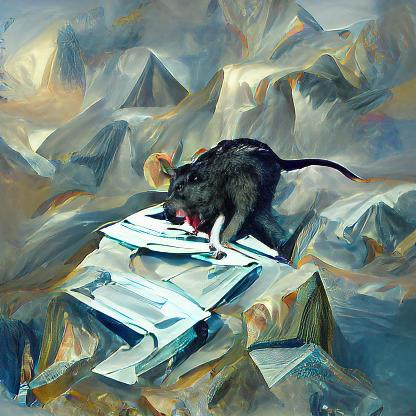
\includegraphics[height=0.6\textheight]{figures/rat_climbing_code_mountain.jpg}\\
    \small ``A tough rat climbing on top of a mountain of program code, oil painting''
  \end{center}
\end{frame}

\begin{frame}
  \frametitle{Mathematisch präzise: Shannon's Entropie}
  \begin{columns}
    \begin{column}{0.4\textwidth}
      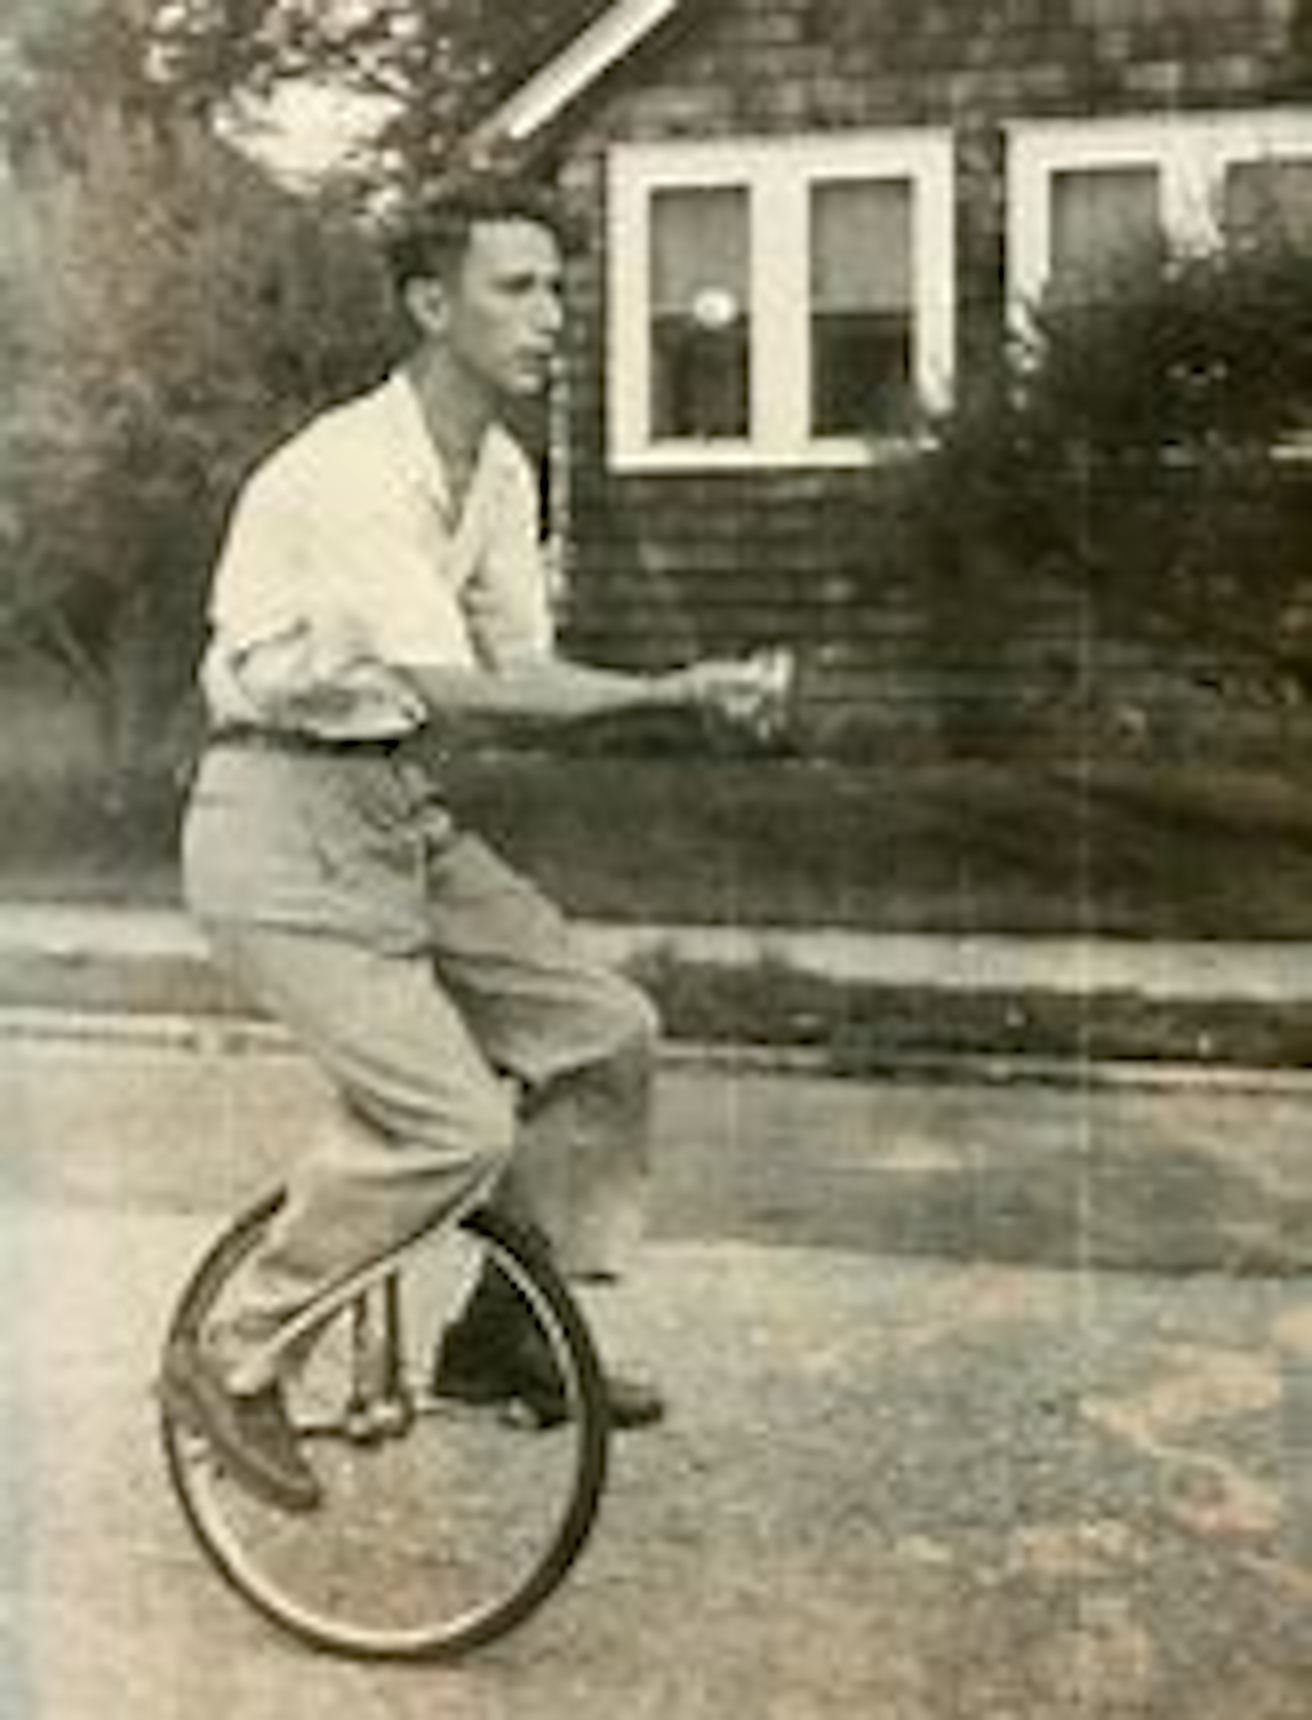
\includegraphics[width=\textwidth]{figures/claude_shannon_unicycle.png}
    \end{column}
    \begin{column}{0.6\textwidth}
      \vspace{-7cm}
      \begin{itemize}[<+->]
        \item \textbf{Claude Shannon (1916--2001)}
        \item 1948: ``A Mathematical Theory of Communication''
        \item Geburt der Informationstheorie.
        \item Mathematische Definition der Entropie (auch ``Information'' oder ``Shannon-Entropie'' genannt).
      \end{itemize}
    \end{column}
  \end{columns}
\end{frame}

\begin{frame}
  \frametitle{Das Setting: eine Nachricht}
  Wir erhalten eine Nachricht in deutscher Sprache, Buchstabe für Buchstabe einzeln.
  \begin{itemize}[<+->]
    \item Wir modellieren jedes einzelne Zeichen als Zufallsvariable
          \[X_n \colon \Omega \to \Sigma\]
          wobei $n$ für das $n$-te Zeichen steht,
    \item und $\Sigma = \{a, b, \dots, z, \textvisiblespace\}$ die Menge der Buchstaben und Leerzeichen bezeichnet -- man nennt das ein \alert{Alphabet}.
  \end{itemize}
  \uncover<3->{
    Wir kennen die deutsche Sprache:
    \begin{itemize}
      \item Wir kennen die Verteilung eines einzelnen $X_n$, z.B. ``e'' ist häufiger als ``y''.
      \item Wir wissen noch mehr: Wenn die ersten 4 Zeichen ``hall'' sind, so ist als fünftes ``o'' deutlich wahrscheinlicher als ``x''.
    \end{itemize}
  }
\end{frame}

\begin{frame}
  \frametitle{Das Setting: eine Nachricht}
  Wir erhalten eine Nachricht in einer Sprache, Buchstabe für Buchstabe einzeln.
  Wir modellieren jedes einzelne Zeichen als Zufallsvariable
  \[X \colon \Omega \to \Sigma\]
  \vspace{-0.5cm}
  \begin{itemize}[<+->]
    \item wobei $\Sigma = \{z_1, z_2, \dots, z_n\}$ ein Alphabet ist
    \item und $p \colon \Sigma \to [0,1]$ die Verteilungsfunktion von $X$, d.h. $p(z) = P(\{z\})$.
    \item Dann ist für jedes Zeichen $z_i$ die \alert{Selbstinformation} bzgl. $X$ definiert als
          \[I_X(z_i) := -\log_2 p(z_i)\]
  \end{itemize}
  \uncover<+->{
    \textbf{Beispiel:} Wenn $p(z_i) = 1/n$ ist, so ist $\log_2 p(z_i) = \log_2(n^{-1}) = -\log_2(n)$, also $I_X(z_i) = \log_2(n)$.\\
    Wenn es $n=32$ Zeichen gibt also $I_X(z_i) = \log_2(32) = 5$.
  }
\end{frame}

\begin{frame}
  \frametitle{Die Entropie $H$}
  \begin{itemize}[<+->]
      \item Die \alert{Entropie $H$} von $X$ ist definiert als der Erwartungswert von $I_X$:
  \[H(X) := \mathbb{E}(I_X) = -\sum_{i} p(z_i) \log_2 p(z_i)\]
 \end{itemize}
\end{frame}


\section{Einschub: Logarithmus}

\begin{frame}
  \frametitle{Logarithmus zur Erinnerung}
  \begin{definition}[Logarithmus]
    Wenn $b, x$ und $y$ reelle Zahlen sind mit der Eigenschaft $b^x = y$, dann heißt $x$ auch \alert{Logarithmus von $y$ zur Basis $b$} und wir schreiben $x = \log_b(y)$.
  \end{definition}
  \begin{itemize}[<+->]
    \item Der Logarithmus zur Basis $e$ (die Eulersche Zahl) heißt auch \alert{natürlicher Logarithmus} und wird mit $\ln = \log_e$ bezeichnet.
    \item Der Logarithmus zur Basis $2$ heißt \alert{binärer Logarithmus} und wird mit $\operatorname{lb} = \log_2$ bezeichnet.
    \item Wegen $10^2 = 100$ und $10^3 = 1000$ wissen wir $\log_{10}(100) = 2$ und $\log_{10}(1000) = 3$.
    \item Weil die Exponentialfunktion monoton wächst, gilt auch für $100 < y < 1000$, dass $2 < \log_{10}(y) < 3$ ist. $\ceil{\log_{10}(y)}$ ist also die Anzahl der Stellen.
  \end{itemize}
\end{frame}

\begin{frame}
  \frametitle{Logarithmus' freundliche Eigenschaften}
  \begin{itemize}[<+->]
    \item Klar: $e^{\ln(y)} = y$ und $x = \ln(e^x)$
    \item Auch gut zu wissen: weil $(e^u)^v = e^{uv}$, gilt:
      \begin{align*}
        b^x &= (e^{\ln(b)})^x = e^{\ln(b)x} \quad \text{(Def. verwenden)} \\
        \ln(b^x) &= \ln(b)x \quad \text{($\ln$ anwenden)} \\
        \ln(y) &= \ln(b)\log_b(y) \quad \text{($x, y$ einsetzen)}
      \end{align*}
    \item Man kann also $\log_b(y)$ als $\frac{\ln(y)}{\ln(b)}$ ausrechnen!
  \end{itemize}
  \uncover<+->{
    \textbf{Beispiel Binär-Logarithmus:} Die Zahl 77 ist in binärer Kodierung \texttt{1001101}.\\
    $1 \cdot 64 + 0 \cdot 32 + 0 \cdot 16 + 1 \cdot 8 + 1 \cdot 4 + 0 \cdot 2 + 1 \cdot 1 = 77$\\
    $\log_2(77) \approx 6.266$
  }
\end{frame}


\section{Zurück zur echten Welt}

\begin{frame}
  \frametitle{Entropie der deutschen Sprache}
  \begin{itemize}[<+->]
    \item Die Entropie der deutschen Sprache lässt sich für einzelne Zeichen ermitteln als \alert{4,0629 bit}.
    \item Wenn man zusätzlich noch betrachtet, wie sich die Wahrscheinlichkeit eines Zeichens ändert, je nachdem was davor für Zeichen stehen, verringert sich die Entropie erheblich, zu ungefähr \alert{1,5 bit} je Buchstaben.
    \item Eine Zeichenkette der Länge 10 über unserem Alphabet mit 26 Buchstaben kann bei Gleichverteilung z.B. so aussehen: \texttt{pashglwnmv} und das enthält pro Zeichen $\approx 4,7$ bit Information, also insgesamt $47$ bit.
    \item Wissen wir hingegen, dass die Zeichenkette ein deutsches Wort ist, z.B. \texttt{kabelkanal}, so liegt der Informationsgehalt nur noch bei $15$ bit. (D.h. mit $2^{15} = 32768$ Versuchen haben wir das Wort erraten.)
  \end{itemize}
  \uncover<+->{
      \vfill
      \tiny Quelle: Fox, D. Entropie. Datenschutz und Datensicherheit - DuD volume 32, 543 (2008).
  }
\end{frame}

\begin{frame}
  \frametitle{Passwörter und Entropie}
  \begin{center}
    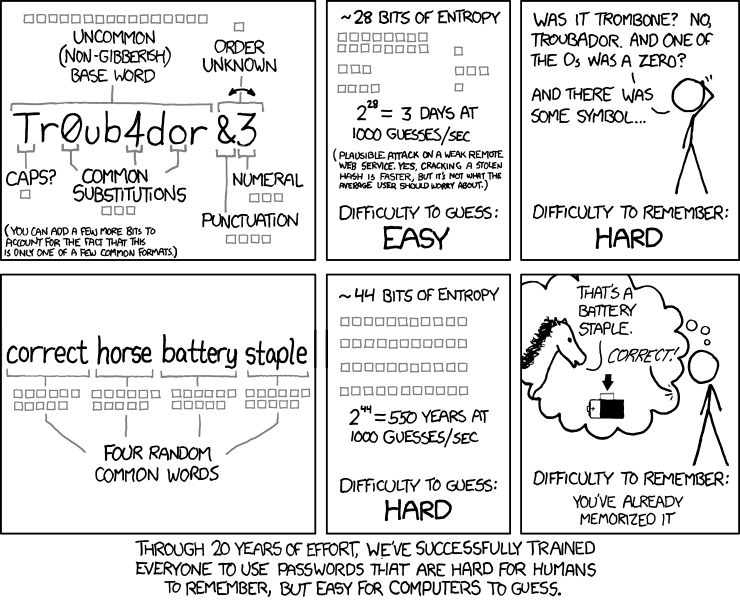
\includegraphics[height=0.7\textheight]{figures/xkcd_password_strength.png}\\
    \tiny Quelle: xkcd.com/936/ (CC BY-NC 2.5)
  \end{center}
\end{frame}

\begin{frame}
  \frametitle{Wo nutzen wir das Konzept ``Entropie''?}
  \textbf{Vor allem bei diesen Kompetenzen:}
  \begin{enumerate}
    \item einen Datensatz explorativ zu analysieren,
    \item Daten zur Weiterverarbeitung zu transformieren,
    \item Teildatensätze zur Weiterverarbeitung zu wählen,
    \item \textbf{geeignete Datensätze zusammenzuführen,}
    \item Erkenntnisse in Daten zu beschreiben und zu visualisieren,
    \item \textbf{statistische Modelle anhand von Daten aufzustellen,}
    \item \textbf{die Güte von Modellen zu bewerten,}
    \item und zur Klassifikation und Vorhersage weiterer Daten zu nutzen.
  \end{enumerate}
\end{frame}


\begin{frame}[separator]
  \frametitle{Zeit für eine Pause?}
  \begin{center}
    
\includegraphics[height=0.5\textheight]{figures/lion_pause.jpg}
  \end{center}
\end{frame}


\section{Diskrete Verteilungen}

\begin{frame}
  \frametitle{Wichtigste diskrete Verteilungen}
  \framesubtitle{Und wie sie gemacht werden}
  \begin{center}
    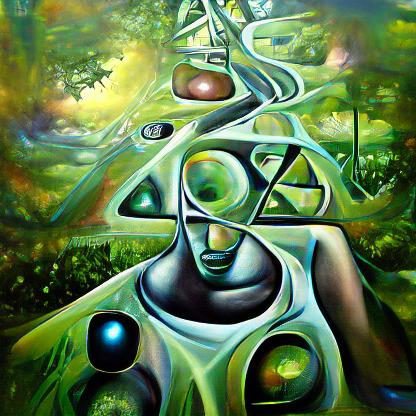
\includegraphics[height=0.6\textheight]{figures/psytrance_enlightenment.jpg}\\
    \small ``The path to mathematical enlightenment, psytrance futuristic, oil canvas''
  \end{center}
\end{frame}

\begin{frame}
  \frametitle{Konvention}
  Sei $\Omega$ ein diskreter Wahrscheinlichkeitsraum, d.h.
  \begin{itemize}[<+->]
    \item $\Omega$ ist eine höchstens abzählbare Menge (oftmals endlich), $\Omega=\{\omega_1, \omega_2, \dots\}$
    \item $\Omega$ trägt die Potenzmenge $\mathcal{P}(\Omega)$ als $\sigma$-Algebra, d.h. alle Mengen von Ergebnissen $A \subseteq \Omega$ sind Ereignisse.
    \item Auf $\Omega$ ist ein Wahrscheinlichkeitsmaß definiert: $P \colon \mathcal{P}(\Omega) \to [0,1]$
    \item Das Wahrscheinlichkeitsmaß ist bereits auf einelementigen Mengen festgelegt:\\
          $p \colon \Omega \to [0,1], \quad p(\omega) := P(\{\omega\})$ \\
          heißt pmf, Verteilungsfunktion, Zähldichte von $P$.
    \item Für eine Zufallsvariable $X \colon \Omega \to \mathbb{R}$ ist $\mathbb{E}X = \sum x p_X(x) = \sum X(\omega)p(\omega)$ der Erwartungswert.
    \item $H(X) = -\sum p(\omega) \log_2(p(\omega))$ die Entropie.
  \end{itemize}
\end{frame}

\begin{frame}
  \frametitle{Diskrete Gleichverteilung}
  \begin{columns}
    \begin{column}{0.6\textwidth}
      \vspace{-2cm}
      \begin{itemize}[<+->]
        \item $p(\omega) = \frac{1}{n}$
        \item $H(X) = \log_2(n)$
        \item $\mathbb{E}(X) = \frac{n+1}{2}$
        \item $\mathbb{V}(X) = \frac{n^2-1}{12}$
        \item \textbf{Standardbeispiel:} fairer Würfel ($n=6$)
      \end{itemize}
    \end{column}
    \begin{column}{0.4\textwidth}
      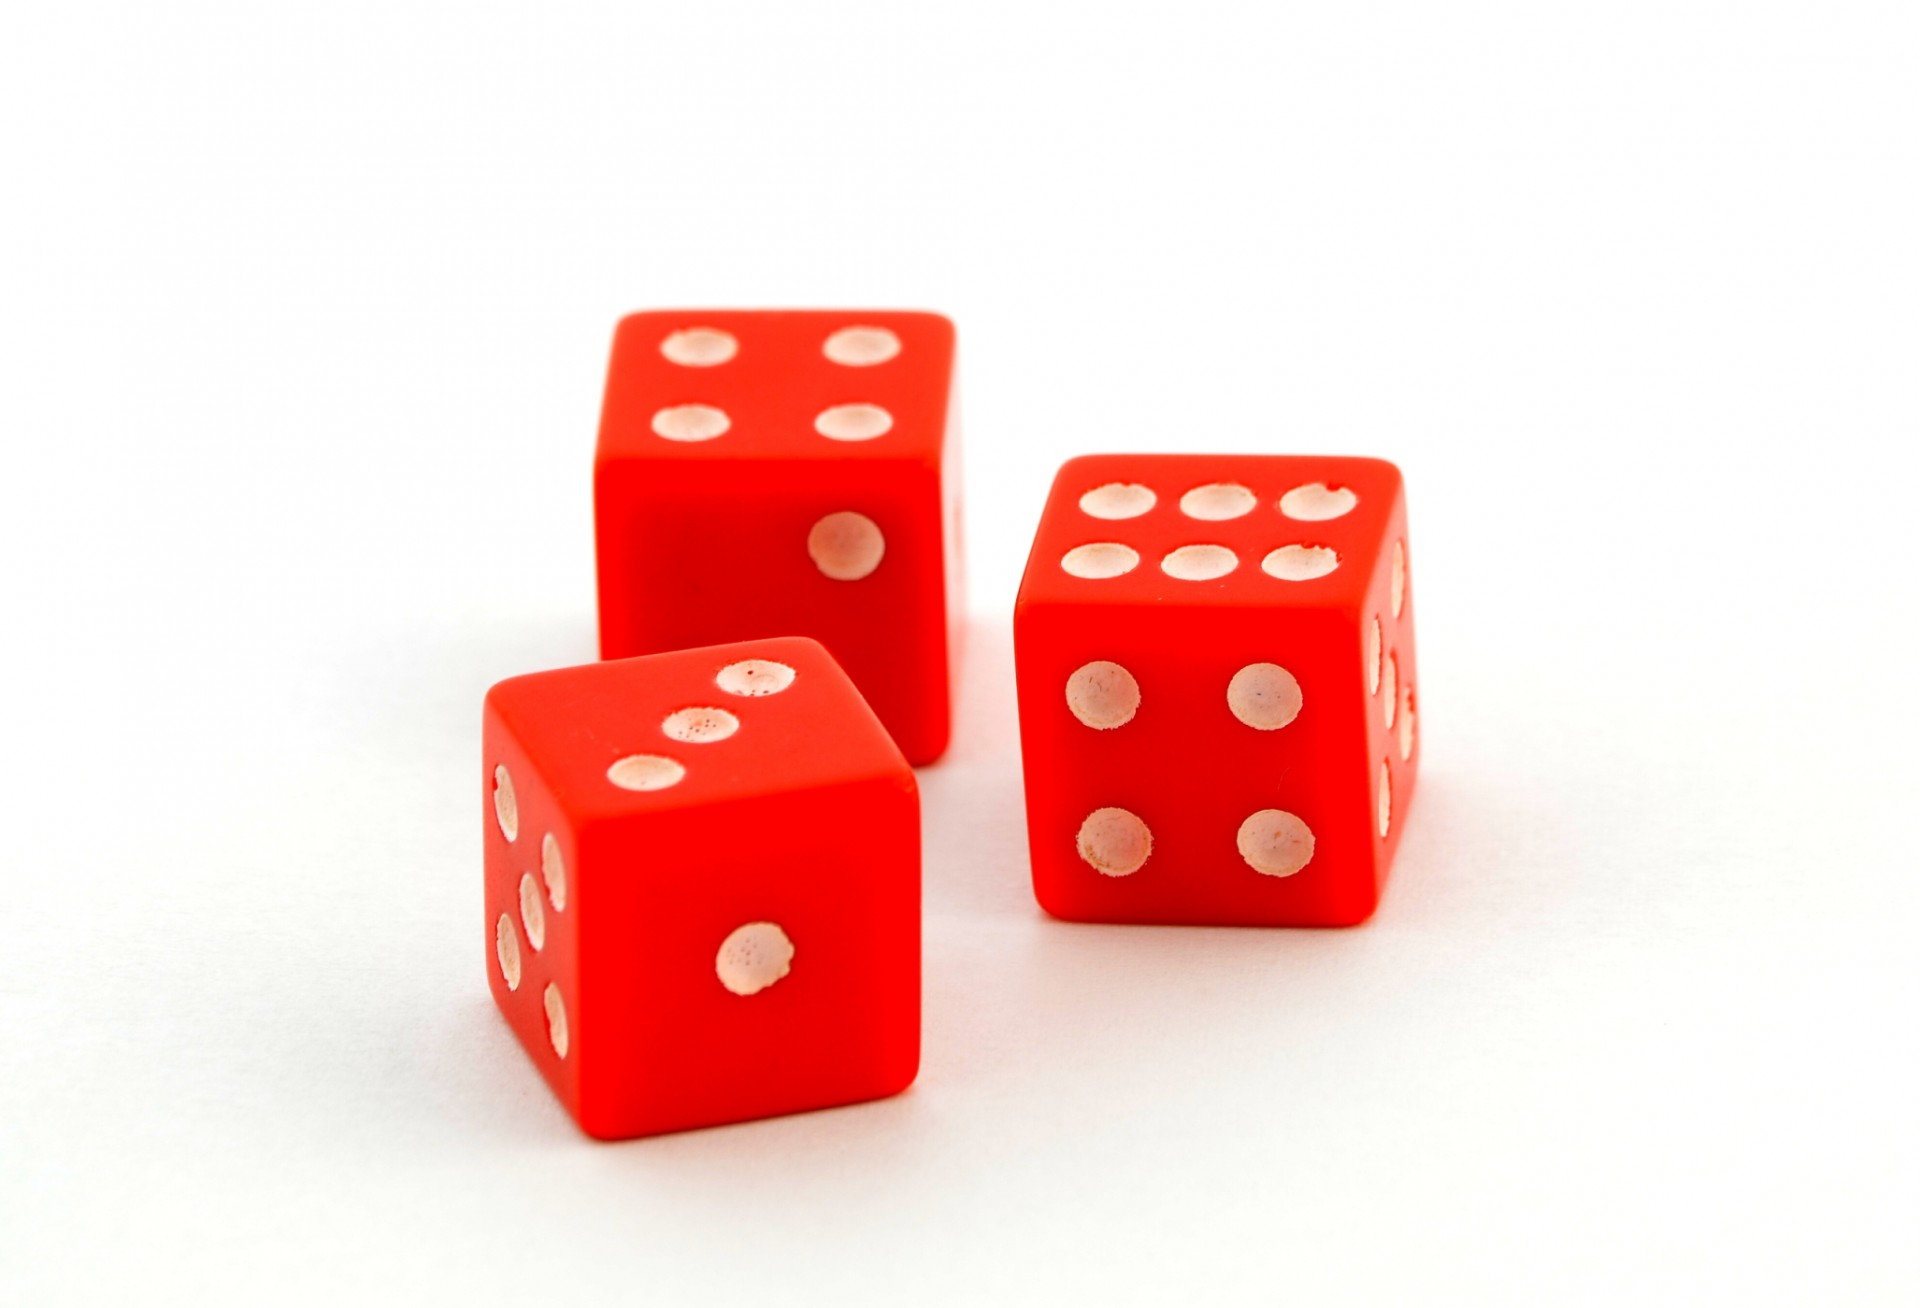
\includegraphics[width=\textwidth]{figures/red_dice.jpg}
    \end{column}
  \end{columns}
\end{frame}

\begin{frame}
  \frametitle{Kategoriale Verteilung}
      \begin{itemize}[<+->]
        \item $p = (p(\omega_i))_{i \ge 1} \in \mathbb{R}^n$ ist ein Vektor, der die Verteilung definiert.
        \item Dabei ist $0 \le p_i \le 1$ und $\sum p_i = 1$.
        \item Der Parameterraum ist ein $(n-1)$-dimensionales Simplex.
        \item Der Mittelpunkt ist $p_1 = p_2 = \dots$, die diskrete Gleichverteilung.
        \item $\mathbb{E}(X) = \sum i p_i$ (i.A. nicht zu vereinfachen).
        \item \textbf{Standardbeispiel:} Urne mit $m$ gefärbten Bällen, $n$ verschiedene Farben, $n_i$ Bälle der Farbe $i$, dann ist $p_i = \frac{n_i}{m}$ und wir ziehen mit Zurücklegen einen Ball.
      \end{itemize}
\end{frame}

\begin{frame}
  \frametitle{Bernoulli-Verteilung}
  Kategoriale Verteilung für $n=2$, $\Omega = \{0,1\}$.
  \begin{columns}
    \begin{column}{0.6\textwidth}
      \vspace{-4cm}
      \begin{itemize}[<+->]
        \item $p = p(1) \in \mathbb{R}$ ist eine Zahl, die die Verteilung definiert.
        \item $\mathbb{E}(X) = p$
        \item $\mathbb{V}(X) = p(1-p)$
        \item $H(X) = -p \log_2(p) - (1-p) \log_2(1-p)$
        \item Die Ableitung nach $p$ der Entropie ist $-\log_2\left(\frac{p}{1-p}\right)$. Nullstelle ist $p = \frac{1}{2}$, also hat der faire Münzwurf maximale Entropie.
        \item \textbf{Standardbeispiel:} Münzwurf mit einer ungleichmäßigen Münze.
      \end{itemize}
    \end{column}
    \begin{column}{0.4\textwidth}
      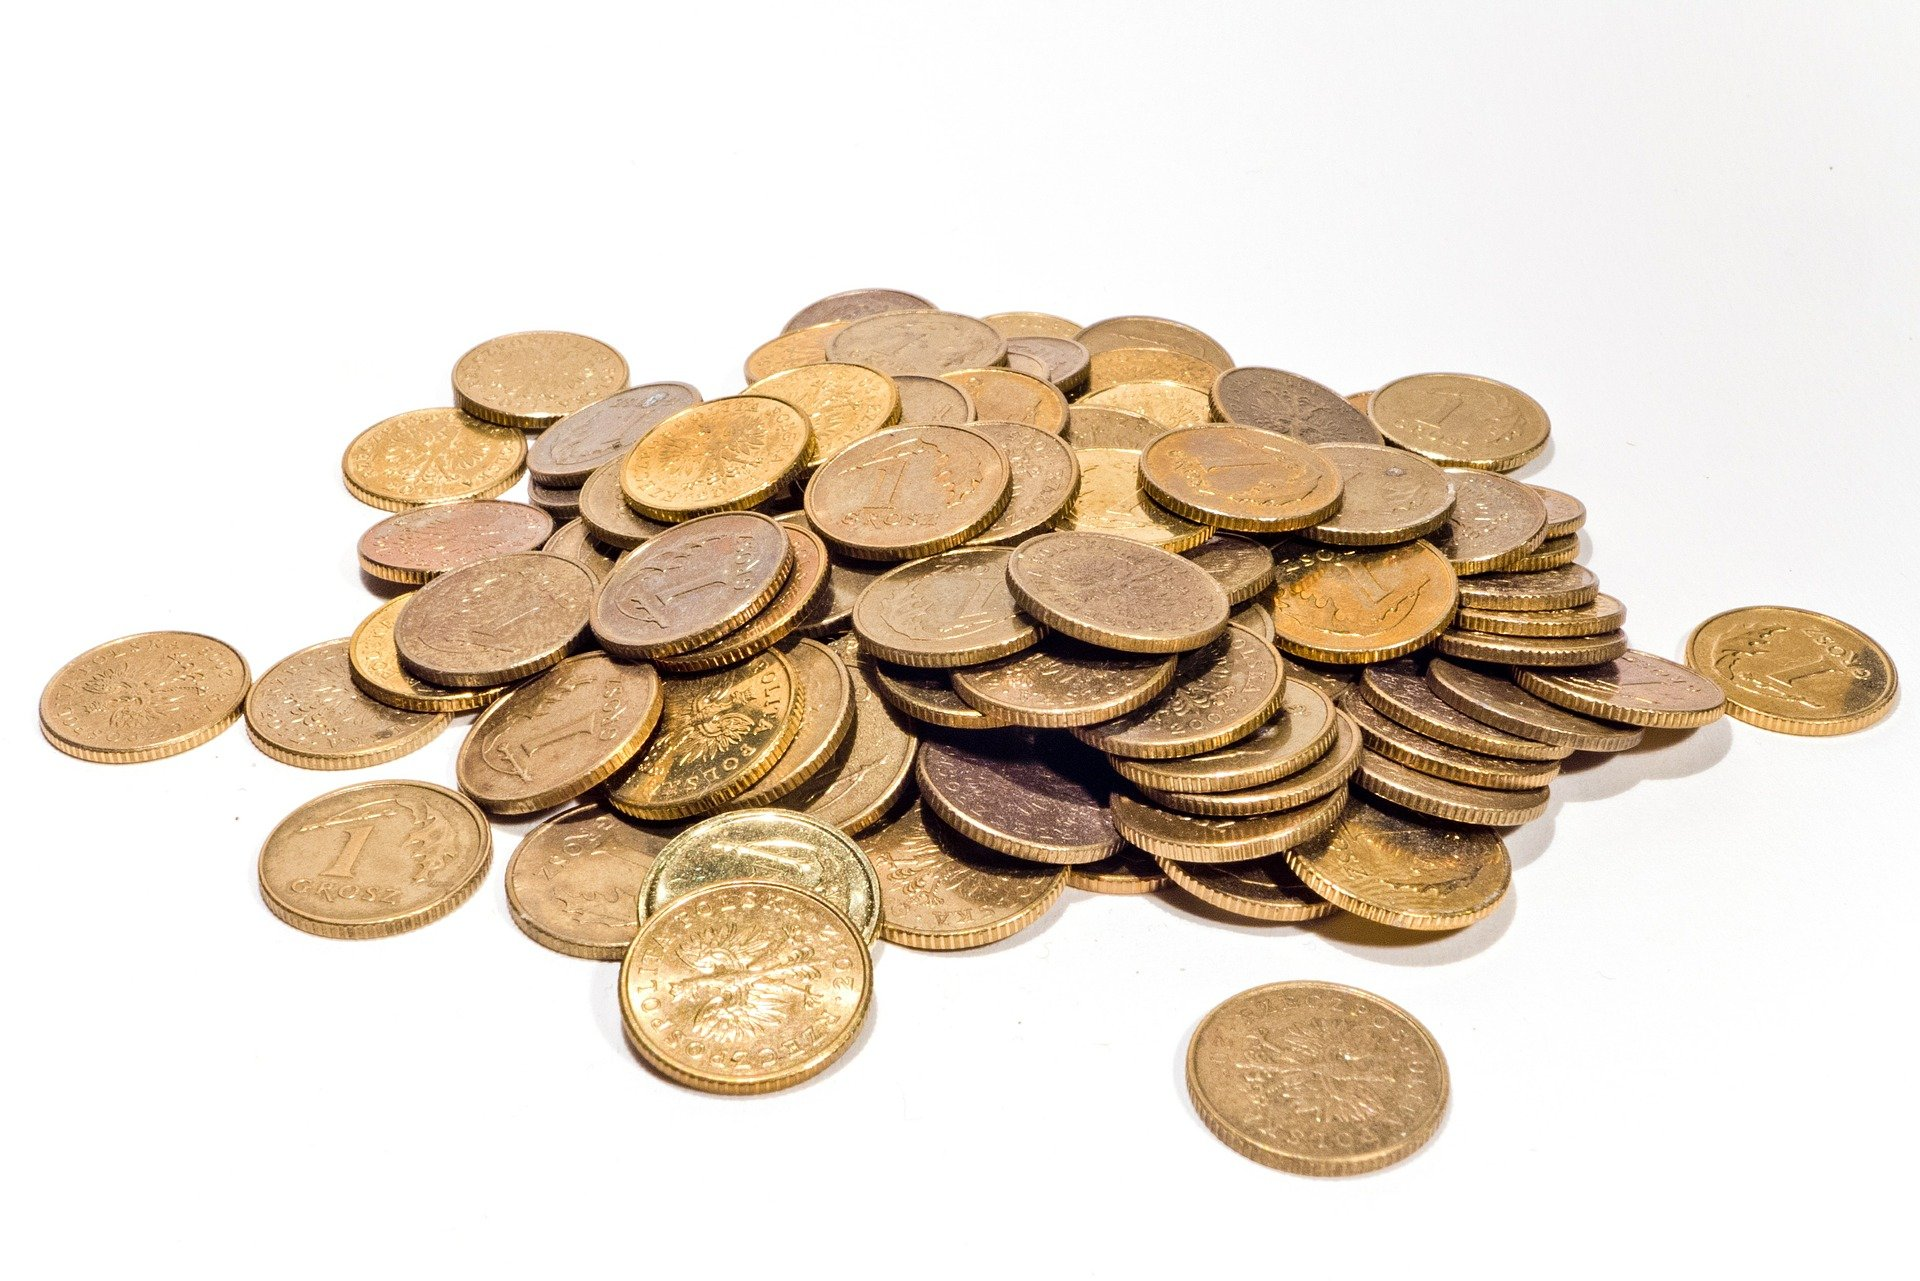
\includegraphics[width=\textwidth]{figures/coins_pile.jpg}
    \end{column}
  \end{columns}
\end{frame}

\begin{frame}
  \frametitle{Binomial-Verteilung}
  Wenn man den Münzwurf (ein Bernoulli-Experiment) mit Parameter $p$ $n$-mal wiederholt und dann die Summe über die Ergebnisse bildet, erhält man eine Zufallsvariable $X \colon \Omega \to \mathbb{R}$.

      \begin{itemize}[<+->]
        \item z.B. mit $\Omega = \{0,1\}^n$
        \item $P(X=k) = \binom{n}{k} p^k (1-p)^{n-k}$
        \item $\mathbb{E}(X) = np$
        \item $\mathbb{V}(X) = np(1-p)$
        \item Man schreibt: $X \sim \operatorname{Bin}(n,p)$
        \item \textbf{Urnenmodell:} zwei verschiedenfarbige Bälle, $p = \frac{n_1}{N}$ und $N = n_1 + n_2$, ziehen mit Zurücklegen.
      \end{itemize}
\end{frame}

\begin{frame}
  \frametitle{Poisson-Binomialverteilung}
  Verallgemeinerung des $n$-fachen Münzwurfs: Für jeden Wurf eine andere Münze (Parameter $p_1, p_2, \dots, p_n$).
  \begin{itemize}[<+->]
    \item $P(X=k) = \sum_{A \in F_k} \prod_{i \in A} p_i \prod_{i \notin A} (1-p_i)$\\
          ($F_k = $ Menge der $k$-elementigen Teilmengen von $\{1,\dots,n\}$)
    \item $\mathbb{E}(X) = \sum p_i$
    \item $\mathbb{V}(X) = \sum (1-p_i)p_i$
    \item $H(X)$ ist kleinergleich der Entropie einer Binomialverteilung ($p_1 = p_2 = \dots$).
  \end{itemize}
  \uncover<+->{
    \vspace{0.2cm}
    Wenn es \alert{unendlich viele} Münzen gibt und die $p_i$ schnell genug kleiner werden ($i \to \infty$), genauer $\lim_{i \to \infty} i p_i = \lambda > 0$, dann lässt sich die Verteilung gut approximieren:
    \[ \lim_{n \to \infty} \binom{n}{k} p_n^k (1-p_n)^{n-k} = e^{-\lambda} \frac{\lambda^k}{k!} \]
  }
\end{frame}

\begin{frame}
  \frametitle{Poissonverteilung}
  In einem festen Zeitintervall, wie viele (unabhängig voneinander mit konstanter mittlerer Rate eintretende) Ereignisse treten ein?

      \begin{itemize}[<+->]
        \item $P(X=k) = e^{-\lambda} \frac{\lambda^k}{k!}$
        \item Dabei ist $k$ die Zahl, wie viele Ereignisse eintreten.
        \item $\mathbb{E}(X) = \lambda$
        \item $\mathbb{V}(X) = \lambda$
      \end{itemize}

\end{frame}


\section{Numpy}

\begin{frame}[separator]
  \frametitle{Einstieg in Numpy}
  \framesubtitle{Schnelle Arrays}
\end{frame}

\begin{frame}
  \frametitle{Numpy Cheat Sheet}
  \begin{center}
    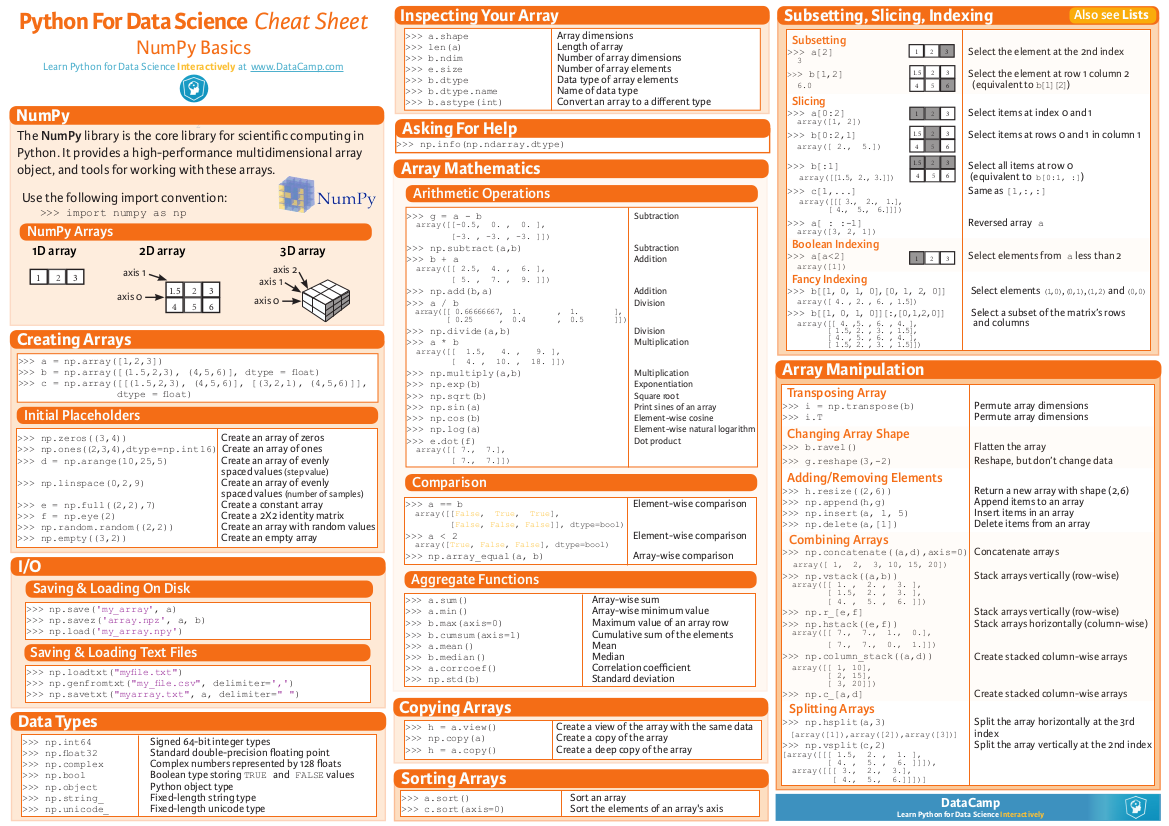
\includegraphics[height=0.8\textheight]{figures/numpy_cheat_sheet.png}
  \end{center}
\end{frame}

\begin{frame}[separator]
  \frametitle{Vielen Dank für Ihre Aufmerksamkeit!}
\end{frame}

\end{document}
%%% Local Variables:
%%% mode: latex
%%% TeX-master: t
%%% End: